\section{What the theorem does and does not identify}
\label{sec:scope}

The theorem proves weak convergence for the explicit finite-source sequence defined in Section~\ref{sec:theorem}. The limiting Borel probability measure is constructed by tightness and subsequential extraction, then uniquely identified through its finite weighted Fourier marginals. The statement is for a two-dimensional periodic carrier, with fixed period $L>0$ and mass $M>0$.

A separate construction in the Lean package starts from the physical lattice Gaussian measure `physicalGJMeasure` and maps its total representative into the same carrier. That map requires a named `PeriodicHMinusThreeLiftMeasureInput` for measurability and almost-everywhere representative agreement. It is not the source of the sequence in Theorem~\ref{thm:main}, and the theorem does not use or discharge that input. Keeping the two maps distinct avoids treating a conditional physical-lattice bridge as part of an unconditional finite-source theorem.

The result does not assert an interacting-field limit, an Osterwalder--Schrader reconstruction, an infinite-volume limit, a theorem in other dimensions, or an identification with a separately specified distribution-space model. The construction provides a measure through Prokhorov compactness and characterizes it by finite Fourier laws; it does not claim a samplewise Fourier-series representation beyond what those statements entail.

\begin{figure}[tb]
  \centering
  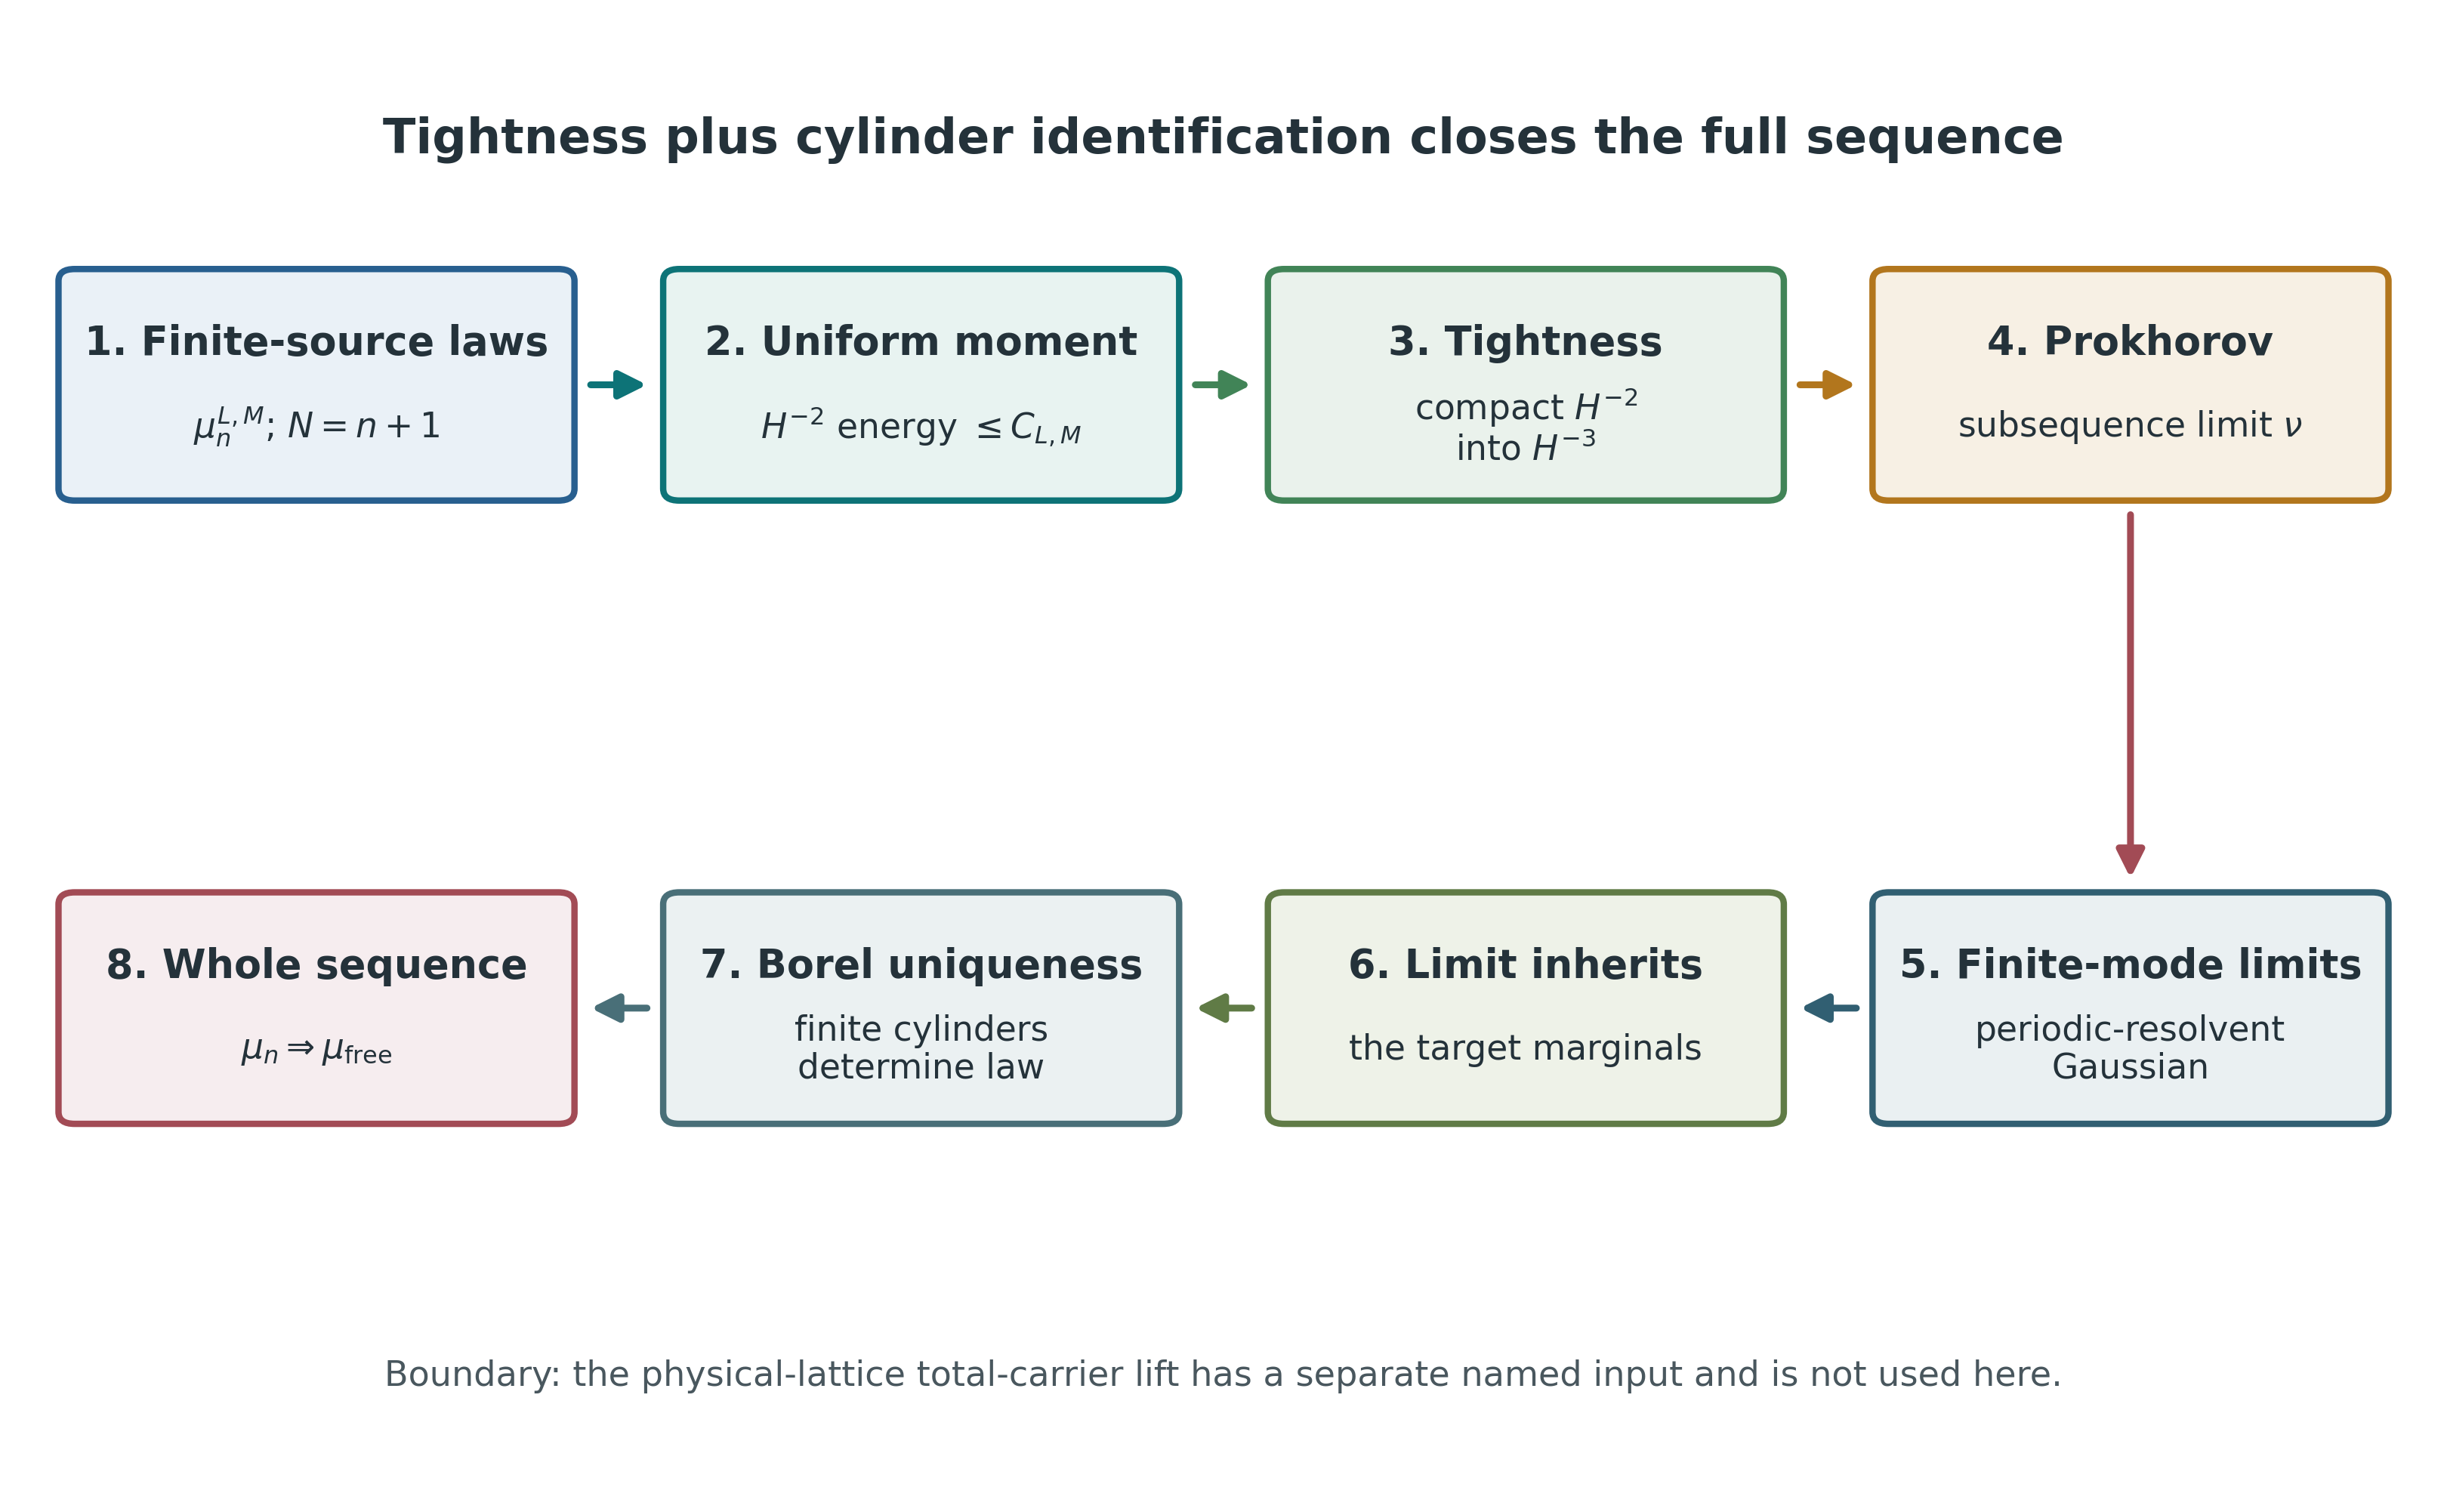
\includegraphics[width=0.98\linewidth]{figures/weak_limit_spine.png}
  \caption{Proof-dependency map for Theorem~\ref{thm:main}. Read the upper row from left to right, then continue from the upper-right box to the lower-right box and follow the lower row back toward the left: the moment bound yields tightness and subsequential limits; finite-mode convergence fixes their Gaussian marginals; Borel cylinder uniqueness identifies all limits and closes whole-sequence convergence. The displayed figure is a generated explanatory diagram, not independent mathematical evidence.}
  \label{fig:proof-spine}
\end{figure}
